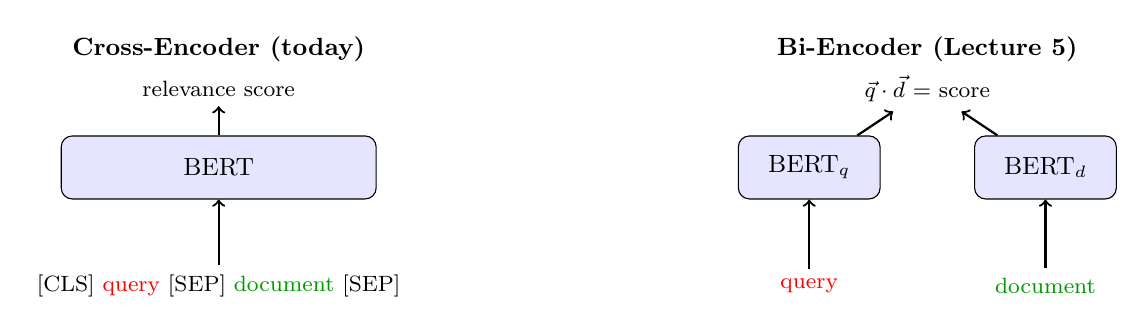
\begin{tikzpicture}[
    box/.style={rectangle, draw, rounded corners, fill=blue!10, minimum height=0.8cm, align=center, font=\small},
    arrow/.style={->, thick}
]
    % Cross-encoder
    \node[font=\small\bfseries] at (-4.5, 3.5) {Cross-Encoder (today)};
    \node[box, minimum width=4cm] (cross_bert) at (-4.5, 2) {BERT};
    \node[font=\footnotesize] (cross_in) at (-4.5, 0.5) {[CLS] \textcolor{red}{query} [SEP] \textcolor{green!60!black}{document} [SEP]};
    \node[font=\footnotesize] (cross_out) at (-4.5, 3) {relevance score};
    \draw[arrow] (cross_in) -- (cross_bert);
    \draw[arrow] (cross_bert) -- (cross_out);

    % Bi-encoder
    \node[font=\small\bfseries] at (4.5, 3.5) {Bi-Encoder (Lecture 5)};
    \node[box, minimum width=1.8cm] (bi_q) at (3, 2) {BERT$_q$};
    \node[box, minimum width=1.8cm] (bi_d) at (6, 2) {BERT$_d$};
    \node[font=\footnotesize, red] (q_in) at (3, 0.5) {query};
    \node[font=\footnotesize, green!60!black] (d_in) at (6, 0.5) {document};
    \node[font=\footnotesize] (dot) at (4.5, 3) {$\vec{q} \cdot \vec{d}$ = score};
    \draw[arrow] (q_in) -- (bi_q);
    \draw[arrow] (d_in) -- (bi_d);
    \draw[arrow] (bi_q) -- (dot);
    \draw[arrow] (bi_d) -- (dot);
\end{tikzpicture}
